\documentclass[12pt]{report}
\usepackage[utf8]{inputenc}
\usepackage[russian]{babel}
%\usepackage[14pt]{extsizes}
\usepackage{listings}
\usepackage[justification=centering]{caption}

% Для листинга кода:
\lstset{ %
language=c++,                 % выбор языка для подсветки (здесь это С)
basicstyle=\small\sffamily, % размер и начертание шрифта для подсветки кода
numbers=left,               % где поставить нумерацию строк (слева\справа)
numberstyle=\tiny,           % размер шрифта для номеров строк
stepnumber=1,                   % размер шага между двумя номерами строк
numbersep=5pt,                % как далеко отстоят номера строк от подсвечиваемого кода
showspaces=false,            % показывать или нет пробелfile:///home/trvehazzk3r/Desktop/test/report.teы специальными отступами
showstringspaces=false,      % показывать или нет пробелы в строках
showtabs=false,             % показывать или нет табуляцию в строках
frame=single,              % рисовать рамку вокруг кода
tabsize=2,                 % размер табуляции по умолчанию равен 2 пробелам
captionpos=t,              % позиция заголовка вверху [t] или внизу [b] 
breaklines=true,           % автоматически переносить строки (да\нет)
breakatwhitespace=false, % переносить строки только если есть пробел
escapeinside={\#*}{*)}   % если нужно добавить комментарии в коде
}

\usepackage{hyperref}
\hypersetup{
    linktoc=all,     %set to all if you want both sections and subsections linked
    linkcolor=blue,  %choose some color if you want links to stand out
}

% Для измененных титулов глав:
\usepackage{titlesec, blindtext, color} % подключаем нужные пакеты
\definecolor{gray75}{gray}{0.75} % определяем цвет
\newcommand{\hsp}{\hspace{20pt}} % длина линии в 20pt
% titleformat определяет стиль
\titleformat{\chapter}[hang]{\Huge\bfseries}{\thechapter\hsp\textcolor{gray75}{|}\hsp}{0pt}{\Huge\bfseries}


% plot
\usepackage{pgfplots}
\usepackage{filecontents}
\usetikzlibrary{datavisualization}
\usetikzlibrary{datavisualization.formats.functions}
\begin{filecontents}{LevRec.dat}
5 10867
7 258961
10 33589820
\end{filecontents}

\begin{filecontents}{LevRecMat.dat}
10 3146
20 12896
30 29325
50 70918
100 184238
200 643895
\end{filecontents}

\begin{filecontents}{LevIterMat.dat}
10 2001
20 4686
30 10744
50 29257
100 86268
200 248651
\end{filecontents}

\begin{filecontents}{DamLev.dat}
10 2137
20 6251
30 13631
50 38427
100 118891
200 299743
\end{filecontents}


\begin{document}
%\def\chaptername{} % убирает "Глава"
\begin{titlepage}
	\fontsize{12pt}{12pt}\selectfont
	\noindent \begin{minipage}{0.15\textwidth}
		
\includegraphics[width=\linewidth]{inc/img/b_logo.jpg}
	\end{minipage}
	\noindent\begin{minipage}{0.9\textwidth}\centering
		\textbf{Министерство науки и высшего образования Российской Федерации}\\
		\textbf{Федеральное государственное бюджетное образовательное учреждение высшего образования}\\
		\textbf{«Московский государственный технический университет имени Н.Э.~Баумана}\\
		\textbf{(национальный исследовательский университет)»}\\
		\textbf{(МГТУ им. Н.Э.~Баумана)}
	\end{minipage}
	
	\noindent\rule{15cm}{3pt}
	\newline\newline
	\noindent ФАКУЛЬТЕТ \underline{~~~~~~~~~~~~~~~~«Информатика и системы управления»~~~~~~~~~~~~~~~~} \newline\newline
	\noindent КАФЕДРА \underline{«Программное обеспечение ЭВМ и информационные технологии»}\newline\newline\newline\newline\newline\newline\newline
	
	
	\begin{center}
		\Large\textbf{Отчет по лабораторной работе №1 по курсу "Анализ алгоритмов"}\newline
	\end{center}
	
	\noindent\textbf{Тема} \underline{Расстояния Левенштейна и Дамерау-Левенштейна}\newline\newline\newline
	\noindent\textbf{Студент} \underline{Якуба Д. В.}\newline\newline
	\noindent\textbf{Группа} \underline{ИУ7-53Б}\newline\newline
	\noindent\textbf{Оценка (баллы)} \underline{~~~~~~~~~~~~~~~~~~~}\newline\newline
	\noindent\textbf{Преподаватели} \underline{Волкова Л.Л., Строганов Ю.В.}\newline
	
	\begin{center}
		\vfill
		Москва~---~\the\year
		~г.
	\end{center}
\end{titlepage}

\tableofcontents

\newpage
\chapter*{Введение}
\addcontentsline{toc}{chapter}{Введение}
\section*{Цель лабораторной работы}
Изучение и реализация алгоритмов нахождения расстояния Левенштейна и Дамерау-Левенштейна.
\section*{Определение}
Расстояние Левенштейна - это мера, определяющая различие двух последовательностей символов. По неформальному определению расстояние Левенштейна между двумя словами - это мимнимальное количество односимвольных изменений (вставок, удалений или замен), необходимых для преобразования одного слова в другое.

Расстояние Левенштейна применяется в теории информации и компьютерной лингвистике для:

\begin{itemize}
	\item Авто-исправления ошибок в слове
	\item Сравнение введёных строк со словарными в поисковых запросах
	\item Сравнения текстовых файлов утилитой diff
	\item В биоинформатике для сравнения генов, хромосом и белков
\end{itemize}

Расстояние Дамерау-Левенштейна - это также мера, определяющая различие двух последовательностей символов, однако набор доступных операций для преобразований строк расширяется - добавляется операция транспозиции (перестановка двух соседствующих символов).

\section*{Задачи лабораторной работы}
Задачами данной лабораторной являются:
\begin{enumerate}
  	\item Изучение алгоритмов Левенштейна и Дамерау-Левенштейна;
	\item Применение метода динамического программирования для реализации указанных алгоритмов; 
	\item Получение практических навыков реализации алгоритмов Левенштейна и Дамерау-Левенштейна; 
	\item Сравнительный анализ реализованных алгоритмов; 
	\item Подготовка отчёта по проведённой работе. 
\end{enumerate}


\chapter{Аналитическая часть}
Расстояние Левенштейна - это минимальное ннобходимое количество операций (вставки, замены, удаления) редакторских операций для преобразования одной строки в другую.

При нахождении расстояния Дамерау — Левенштейна добавляется операция транспозиции (перестановки соседствующих символов).  
 
\textbf{Обозначение редакторских операций:} 
\begin{enumerate}
	\item I - вставка символа;
	\item R - замена символа;
	\item D - удаление символа;
	\item M - бездействие (совпадение символов);
\end{enumerate}

При этом для каждой операции задаётся своя цена (или штраф). Для решения задачи необходимо найти последовательность операций, минимизирующую суммарную цену всех проведённых операций. При этом следует отметить, что:
\begin{enumerate}
	\item $price(x, x) = 0$ - цена замены символа $x$ самого на себя;
	\item $price(x, y) = 0$   $(x \neq y)$ - цена замены символа $x$ на символ $y$;
	\item $price(\alpha, x)$ - цена вставки символа $x$;
	\item $price(x, \alpha)$ - цена удаления символа $x$.
\end{enumerate}

\section{Рекурсивный алгоритм нахождения расстояния Левенштейна}
Пусть $s_{1}$ и $s_{2}$ — две некоторые строки. Тогда расстояние Левенштейна может быть вычислено по формуле \ref{recAlg}

\begin{equation}
\label{recAlg}
\begin{displaymath}
D(i,j) = \left\{ \begin{array}{ll}
 0 & \textrm{$i = 0, j = 0$}\\
 i & \textrm{$j = 0, i > 0$}\\
 j & \textrm{$i = 0, j > 0$}\\
min(\\
D(i,j-1)+1\\
D(i-1, j) +1 &\textrm{$j>0, i>0$}\\
D(i-1, j-1) + m(s_{1}[i], s_{2}[j])\\
)
  \end{array} \right.
  \end{equation}
\end{displaymath}
где функция $m(x,y)$ ($x$ и $y$ - символы) равна нулю, если $a=b$, и единице в противном случае; $x[i]$ - это $i$-ый символ строки $x$.

При этом очевидны следующие факты:
\begin{enumerate}
	\item $D(s_{1}, s_{2})$ \geq $ ||s_{1}| - |s_{2}||$
	\item $D(s_{1}, s_{2})$ \leq $ max(|s_{1}|, |s_{2}|)$
	\item $D(s_{1}, s_{2}) = 0$ \Leftrightarrow $ s_{1} = s_{2}$
\end{enumerate}

Суть рекурсивного алгоритма заключается в реализации формулы \ref{recAlg}.

\section{Рекурсивный алгоритм нахождения расстояния Левенштейна с использованием матрицы}
Для оптимизации рекурсивного алгоритма нахождения расстояния Левенштейна допустимо добавить матрицу для хранения значений $D(i, j)$ для того, чтобы не вычислять их заново раз за разом. Таким образом, при обработке ещё не затронутых данных, результат нахождения расстояния будет занесён в матрицу расстояний. В ином случае, если для рассматриваемого случая информация о расстоянии уже присутствует в матрице, алгоритм будет переходить к следующему шагу.

\section{Итеративный алгоритм нахождения расстояния Левенштейна с использованием матрицы}
Данный алгоритм также заключается в решении задачи с использованием матрицы расстояний. От уже рассмотренного рекурсивного алгоритма нахождения расстояния Левенштейна с использованием матрицы итеративный алгоритм заключается в построчном заполнении матрицы последовательно вычисляемыми $D(i, j)$.

\section{Алгоритм нахождения расстояния Дамерау-Левенштейна с использованием матрицы}

Расстояние Дамерау-Левенштейна вычисляется по следующей рекуррентной формуле:

\begin{displaymath}\\
\begin{equation}
\label{DLalg}
D(i,j) = \left\{ \begin{array}{ll}
 0, & \textrm{$i = 0, j = 0$}\\
 i, & \textrm{$j = 0, i > 0$}\\
 j, & \textrm{$i = 0, j > 0$}\\
min(\\
D(i,j-1)+1,\\
D(i-1, j) +1, &\textrm{$j>0, i>0$}\\
D(i-1, j-1) + m(s_{1}[i], s_{2}[j])\\
D(i-2, j-2) + 1, &\textrm{$i,j>1$, $s_{1}[i] = s_{2}[j-1],s_{1}[i-1]=s_{2}[j] $}\\
)
  \end{array} \right.
  \end{equation}
\end{displaymath}

Применение данной формулы для реализации рекурсивного алгоритма при больших значениях $i, j$ будет работать достаточно долго по тем же причинам, что и реализация рекурсивного алгоритма поиска расстояния Левенштейна. По этой причине целесообразно ввести матрицу, в которой будут храниться вычисленные по формуле значения.

\section{Вывод}
Для каждого рассмотренного алгоритма имеется некоторая рекуррентная формула, что даёт возможность изучить как рекурсивные, так и итеративные реализации алгоритмов. Для оптимизации рекурсивных алгоритмов в рассмотрение вводится матрица, в которую записываются все промежуточные вычисленные значения. Эта же матрица применяется и при реализации итеративных алгоритмов.

\newpage

\chapter{Конструкторская часть}
\section{Блок-схема рекурсивного алгоритма Левенштейна}
Блок-схема рекурсивного алгоритма поиска расстояния Левенштейна предоставлена на рисунке \ref{KC:1}.
\section{Блок-схема рекурсивного алгоритма Левенштейна с использованием матрицы}
Блок-схема рекурсивного алгоритма поиска расстояния Левенштейна с использованием матрицы расстояний предоставлена на рисунке \ref{KC:2}.
\section{Блок-схема итеративного алгоритма Левенштейна}
Блок-схема итеративного алгоритма поиска расстояния Левенштейна с использованием матрицы расстояний предоставлена на рисунке \ref{KC:3}.
\section{Блок-схема алгоритма Дамерау-Левенштейна}
Блок-схема алгоритма поиска расстояния Дамерау-Левенштейна предоставлена на рисунке \ref{KC:4}.
\begin{figure}
\begin{center}

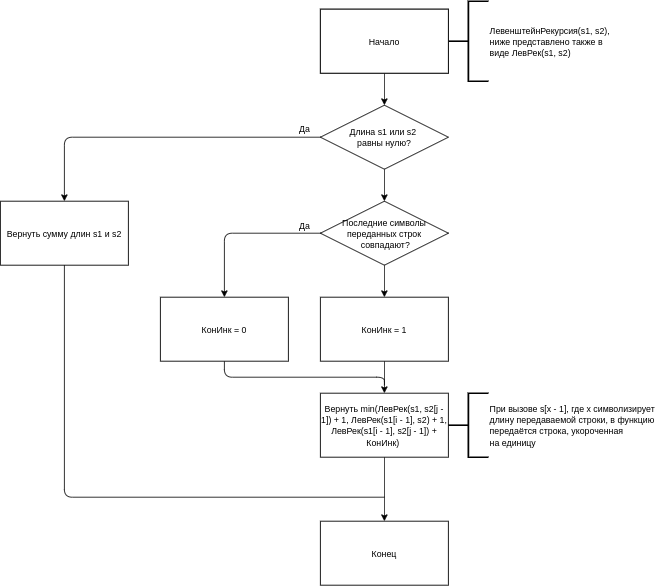
\includegraphics[scale=0.75]{inc/img/LevRec.png}{}
\captionsetup{justification=centering}
	\caption{Блок-схема, описывающая работу рекурсивного алгоритма поиска расстояния Левенштейна.}
	\label{KC:1}
\end{center}
\end{figure}
\begin{figure}
\begin{center}
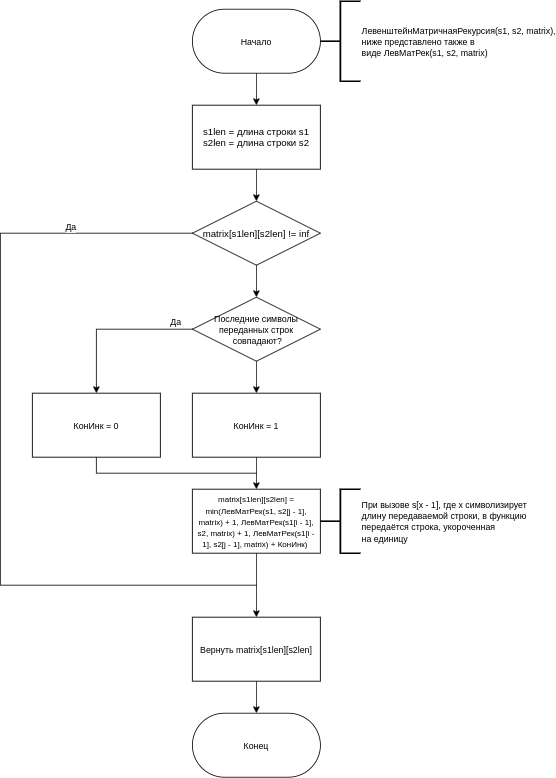
\includegraphics[scale=0.65]{inc/img/LevMatrRec.png}{}
\captionsetup{justification=centering}
	\caption{Блок-схема, описывающая работу рекурсивного алгоритма поиска расстояния Левенштейна с использованием матрицы расстояний.}
	\label{KC:2}
\end{center}
\end{figure}

\begin{figure}
\begin{center}
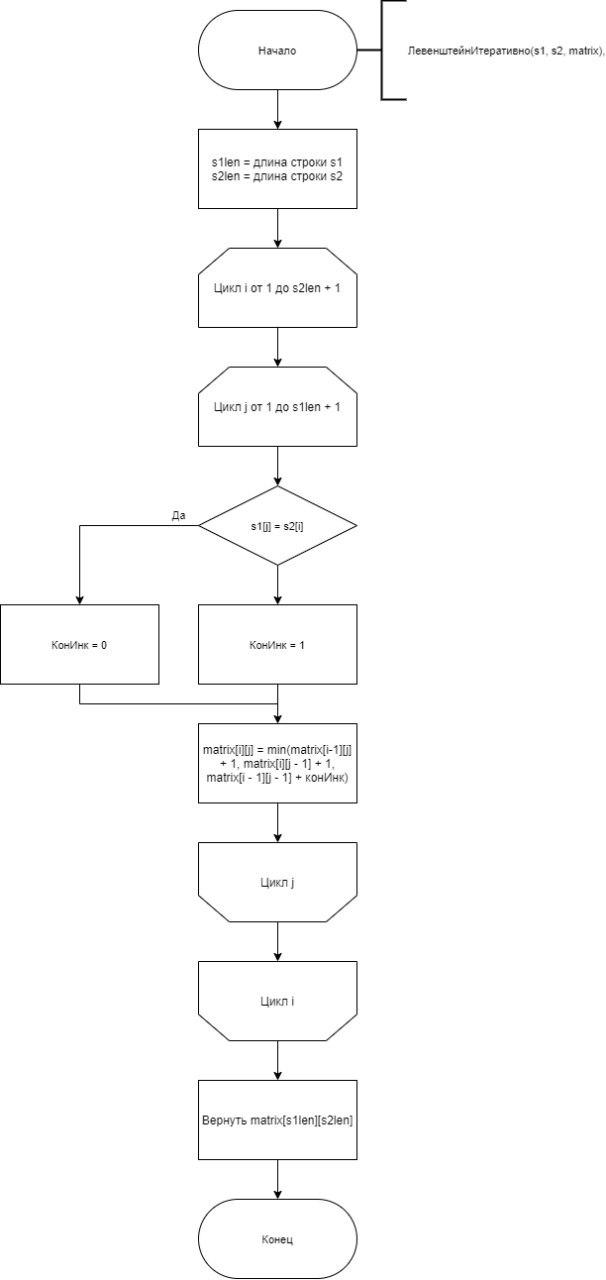
\includegraphics[scale=0.5]{inc/img/LevIter.jpg}{}
\captionsetup{justification=centering}
	\caption{Блок-схема, описывающая работу итеративного алгоритма поиска расстояния Левенштейна с использованием матрицы расстояний.}
	\label{KC:3}

\end{center}
\end{figure}

\begin{figure}
\begin{center}
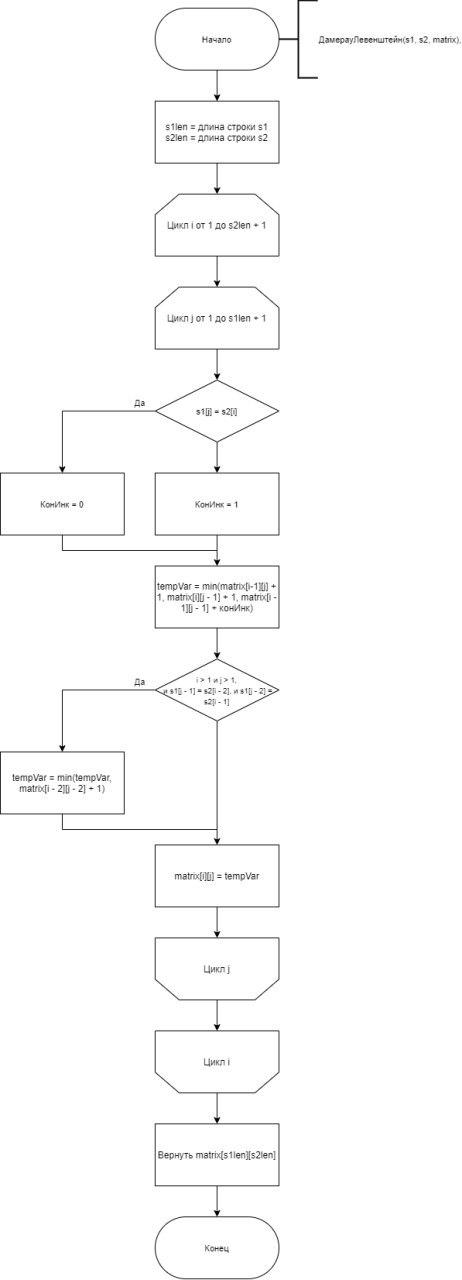
\includegraphics[scale=0.54]{inc/img/DamLev.jpg}{...}
\captionsetup{justification=centering}
	\caption{Блок-схема, описывающая работу алгоритма поиска расстояния Дамерау-Левенштейна.}
	\label{KC:4}

\end{center}
\end{figure}

\chapter{Технологическая часть}
\section{Требования к программному обеспечению}
\begin{itemize}
\item Входные данные - две строки в любой раскладке;
\item Выходные данные - искомое расстояние для выбранного метода и матрица расстояний для методов с её использованием.
\end{itemize}
\section{Средства реализации программного обеспечения}
При написании программного продукта был использован язык программирования C++.

Данный выбор обусловлен следующими факторами:
\begin{itemize}
\item Данный язык программирования преподавался в рамках курса объектно-ориентированного программирования;
\item Высокая вычислительная производительность;
\item Большое количество справочной литературы.
\end{itemize}

Для тестирования производительности реализаций алгоритмов использовалась утилита QueryPerfomanceCounter, объявленная в заголовочном файле "windows.h".

При написаннии программного продукта использовалась среда разработки QT Creator.

Данный выбор обусловлен следующими факторами:
\begin{itemize}
\item Основы работы с данной средой разработки преподавался в рамках курса программирования на Си;
\item QT Creator позволяет работать с расширением QtDesign, которое позволяет создать удобный интерфейс для программного продукта в сжатые сроки.
\end{itemize}

\section{Листинг кода}
В листингах \ref{levRecList} - \ref{DamLevList} предоставлены реализации рассматриваемых алгоритмов.
\begin{lstlisting}[caption=Функция реализации рекурсивного алгоритма Левенштейна,
label={levRecList}]
size_t MainWindow::levenshteinRecursive(QString fWord, QString sWord)
{
    if (!fWord.size() || !sWord.size())
        return fWord.size() + sWord.size();

    return std::min({levenshteinRecursive(fWord, sWord.mid(0, sWord.size() - 1)) + 1,
    levenshteinRecursive(fWord.mid(0, fWord.size() - 1), sWord) + 1,
    levenshteinRecursive(fWord.mid(0, fWord.size() - 1), sWord.mid(0, sWord.size() - 1)) +
    ((fWord.back() == sWord.back()) ? 0 : 1)});
}
\end{lstlisting}

\begin{lstlisting}[caption=Функция реализации рекурсивного алгоритма Левенштейна с использованием матрицы расстояний,
label={levRecMatList}]
size_t MainWindow::levenshteinRecursiveMatrix(
QString fWord, QString sWord, std::vector<std::vector<int>> &matrix)
{
    if (matrix[sWord.size()][fWord.size()] != std::numeric_limits<int>().max())
        return matrix[sWord.size()][fWord.size()];

    matrix[sWord.size()][fWord.size()] =
    std::min({levenshteinRecursiveMatrix(fWord.mid(0, fWord.size() - 1), sWord, matrix) + 1,
    levenshteinRecursiveMatrix(fWord, sWord.mid(0, sWord.size() - 1), matrix) + 1,
    levenshteinRecursiveMatrix(
    fWord.mid(0, fWord.size() - 1), sWord.mid(0, sWord.size() - 1), matrix) +
    ((fWord.back() == sWord.back()) ? 0 : 1)});

    return matrix[sWord.size()][fWord.size()];
}
\end{lstlisting}

\begin{lstlisting}[caption=Функция реализации итеративного алгоритма Левенштейна,
label={levIterList}]
size_t MainWindow::levenshteinNonRecursiveMatrix(
QString fWord, QString sWord, std::vector<std::vector<int>> &matrix)
{
    for (int i = 1; i <= sWord.size(); i++)
        for (int j = 1; j <= fWord.size(); j++)
            matrix[i][j] = std::min({matrix[i - 1][j] + 1, matrix[i][j - 1] + 1,
            matrix[i - 1][j - 1] +
            (((fWord.mid(0, j)).back() == sWord.mid(0, i).back()) ? 0 : 1)});

    return matrix[sWord.size()][fWord.size()];
}
\end{lstlisting}

\begin{lstlisting}[caption=Функция реализации алгоритма Дамерау-Левенштейна,
label={DamLevList}]
bool canBeTranspose(QString fStr, QString sStr, size_t i, size_t j)
{
    return fStr.at(j - 1) == sStr.at(i - 2) && fStr.at(j - 2) == sStr.at(i - 1);
}

size_t MainWindow::damerauLev(
QString fWord, QString sWord, std::vector<std::vector<int>> &matrix)
{
    for (int i = 1; i <= sWord.size(); i++)
        for (int j = 1; j <= fWord.size(); j++)
        {
            int temp = std::min({matrix[i - 1][j] + 1, matrix[i][j - 1] + 1,
            matrix[i - 1][j - 1] +
            (((fWord.mid(0, j)).back() == sWord.mid(0, i).back()) ? 0 : 1)});
            if (i > 1 && j > 1 && canBeTranspose(fWord, sWord, i, j))
                temp = std::min(temp, matrix[i - 2][j - 2] + 1);
            matrix[i][j] = temp;
        }
    return matrix[sWord.size()][fWord.size()];
}
\end{lstlisting}

\section{Тестирование программного продукта}
В таблице \ref{table} приведены тестовые данные и вывод программы для алгоритмов вычисления расстояния Левенштейна и Дамерау-Левенштейна. Тесты пройдены успешно.

\newpage
\begin{table}[h]
	\begin{center}
		\caption{\label{table} Тесты}
		\begin{tabular}{|c|c|c|c|}
	\hline
			                    &                    & \multicolumn{2}{c|}{\bfseries Ожидаемый результат}    \\ \cline{3-4}\hline
	Строка 1& Строка 2 & Алг. Левенштейна & Алг. Дамерау-Левенштейна \\ [0.5ex] 
 	\hline\hline
 	table & tumbler & 3 & 3\\
 	\hline
 	hell & help & 1 & 1\\
 	\hline
	KillUsAll & KlilUsAll & 2 & 1\\
	\hline
	smoke & mssql & 5 & 4\\
	\hline
	OfMiceAndMen & OfMonstersAndMen & 6 & 6\\
	\hline
	roofer & killer & 4 & 4\\
	\hline
	orange & orangina & 3 & 3\\
	\hline
	prolifer & profiler & 2 & 2\\
	\hline
	cat & dog & 3 & 3\\
	\hline
		\end{tabular}
	\end{center}
\end{table}

\section{Вывод}
Спроектированные алгоритмы вычисления расстояния Левенштейна рекурсивно, рекурсивно с использованием матрицы расстояний, итеративно с использованием матрицы расстояний, а также алгоритм вычисления расстояния Дамерау-Левенштейна итеративно с использованием матрицы были реализованы и протестированы.

\chapter{Исследовательская часть}

\section{Пример работы программного обеспечения}
Ниже на рисунках \ref{TD:2} - \ref{TD:5} предоставлены csv-таблицы, сгенерированные по окончанию работы каждого из алгоритмов при передаче строк, описанных на рисунке \ref{TD:1}.

\begin{figure}
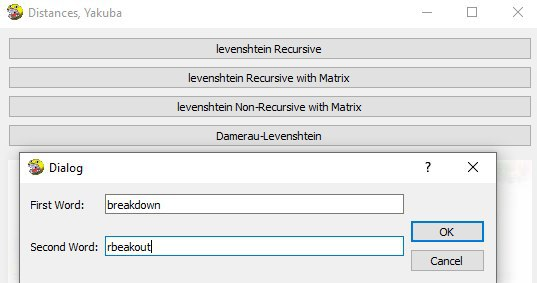
\includegraphics[width=\linewidth]{inc/img/input.png}{
\captionsetup{justification=centering}
	\caption{Передача тестовых данных в ПО.}
	\label{TD:1}
\end{figure}

\begin{figure}
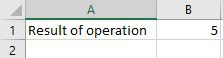
\includegraphics[width=\linewidth]{inc/img/RecAnsw.png}{\newline \textbf{}}
\captionsetup{justification=centering}
	\caption{Итоговая таблица для рекурсивной реализации поиска расстояния Левенштейна.}
	\label{TD:2}
\end{figure}

\begin{figure}
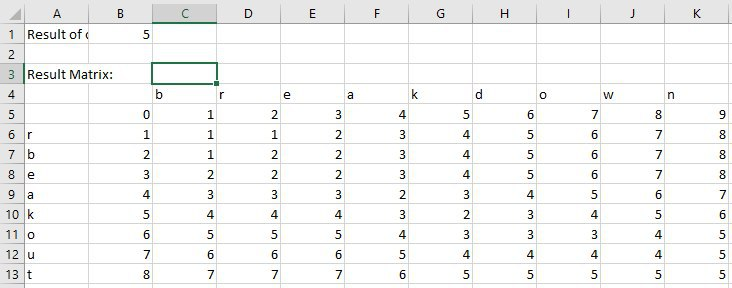
\includegraphics[width=\linewidth]{inc/img/RecMatAnsw.png}{\newline \textbf{}}
\captionsetup{justification=centering}
	\caption{Итоговая таблица для рекурсивной реализации поиска расстояния Левенштейна с использованием матрицы расстояний.}
	\label{TD:3}
\end{figure}

\begin{figure}
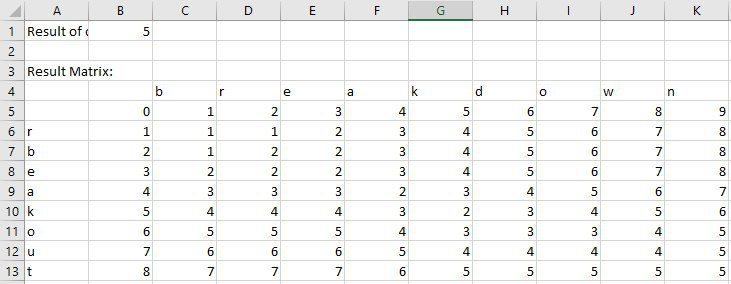
\includegraphics[width=\linewidth]{inc/img/IterMatAnsw.png}{\newline \textbf{}}
\captionsetup{justification=centering}
	\caption{Итоговая таблица для итеративной реализации поиска расстояния Левенштейна с использованием матрицы расстояний.}
	\label{TD:4}
\end{figure}

\begin{figure}
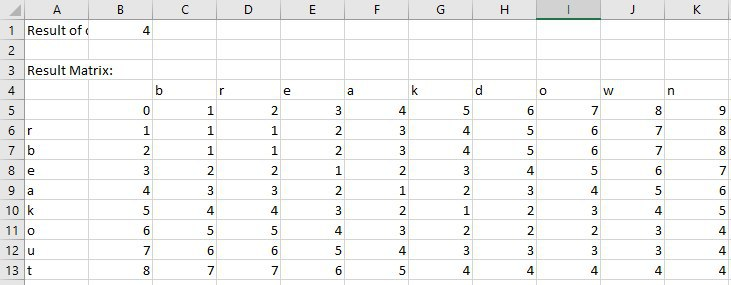
\includegraphics[width=\linewidth]{inc/img/DamLevAnsw.png}{\newline \textbf{}}
\captionsetup{justification=centering}
	\caption{Итоговая таблица для реализации поиска расстяния Дамерау-Левенштейна.}
	\label{TD:5}
\end{figure}

\newpage

\section{Технические характеристики}
Технические характеристики ЭВМ, на котором выполнялись исследования:
\begin{itemize}
\item ОС: Windows 10
\item Оперативная память: 16 Гб
\item Процессор: Intel Core i7-10510U

При проведении замеров времени ноутбук был подключен к сети электропитания.
\end{itemize}

\section{Время выполнения алгоритмов}
Алгоритмы тестировались данных, сгенерированных случайным образом один раз. При увеличении количества символов во входных данных - к уже сгенерированным строкам прибавлялись новые сгенерированные символы.

Тестовые данные:
\begin{itemize}
\item 5 символов:\newline
VxgtU (строка 1),\newline
jRMFA (строка 2)
\item 7 символов:\newline
VxgtUsx (строка 1),\newline
jRMFAyC (строка 2)
\item 10 символов:\newline
VxgtUsx2u3 (строка 1),\newline
jRMFAyCfiV (строка 2)
\item 20 символов:\newline
VxgtUsx2u39dtX81sxy8 (строка 1),\newline
jRMFAyCfiVxyhmILtGMG (строка 2)
\item 30 символов:\newline
VxgtUsx2u39dtX81sxy8GInrYeVNmJ (строка 1),\newline
jRMFAyCfiVxyhmILtGMG4IVZTjPQ7l (строка 2)
\item 50 символов:\newline
VxgtUsx2u39dtX81sxy8GInrYeVNmJvvG7WkaA7Qjs82qP6bJG (строка 1),\newline jRMFAyCfiVxyhmILtGMG4IVZTjPQ7laMIEG6xv9zbdXq9WcJY2 (строка 2)
\item 100 символов:\newline
VxgtUsx2u39dtX81sxy8GInrYeVNmJvvG7WkaA7Qjs82qP6bJG\newline
Ooryez5fYpJWcPRhm7TEjeUoD49M26XDt CJrGtjJXf3aZ9La9n (строка 1),\newline jRMFAyCfiVxyhmILtGMG4IVZTjPQ7laMIEG6xv9zbdXq9WcJY2\newline
G4J0JV1XP8ecmHkTYdY1uzSm8WFY3KjgG ggAw3GrPISl76Mzb1 (строка 2)
\item 200 символов:\newline
VxgtUsx2u39dtX81sxy8GInrYeVNmJvvG7WkaA7Qjs82qP6bJGO\newline
oryez5fYpJWcPRhm7TEjeUoD49M26XDtCJrGtjJXf3aZ9La9nsh\newline
v3cAbwuAJuKc00ndp6EWNHQcArjwXQzAtdpnHs2uOF1kfhWjzXU\newline
S44zKnHVNCaeLyzBlce3RCdGwbJx8s2SlfvYoyBZsKrN1cX (строка 1),\newline
jRMFAyCfiVxyhmILtGMG4IVZTjPQ7laMIEG6xv9zbdXq9WcJY2G\newline
4J0JV1XP8ecmHkTYdY1uzSm8WFY3KjgGggAw3GrPISl76Mzb1f3\newline
ElDEyOeorQGS6CxLWS3lH8sNgZta9vSDMLvnbPaXP24H5dYkBXL\newline
RruvzSlLs1T8hyezy0U3awz65ctATEclCBG4H1pC9mMusWF (строка 2)
\end{itemize}

Результаты замеров времени приведены в таблице \ref{time}. Прочерк в таблице означает, что для заданных значений тестирование не проводилось. На рисунках \ref{recTime}, \ref{IterTime} приведены графики зависимостей времени работы алгоритмов от длины строк, подаваемых на вход.

\begin{table}[h]
	\begin{center}
		\caption{\label{time} Замеры времени для строк различной длины}
		\begin{tabular}{|c c c c c|} 
 			\hline
			Длина строк & LevRec & LevMatRec & LevMatIter & DamLev \\ [0.5ex] 
 			\hline\hline
 			5 & 10867 & - & - & -\\
 			\hline
 			7 & 258961 & - & - & -\\
 			\hline
			10 & 33589820 & 3146 & 2001 & 2137\\
			\hline
			20 & - & 12896 & 4686 & 6251\\
			\hline
			30 & - & 29325 & 10744 & 13631\\
			\hline
			50 & - & 70918 & 2927 & 38427\\
			\hline
			100 & - & 184238 & 86268 & 118891\\
			\hline
			200 & - & 642895 & 248651 & 299743\\
			\hline
			\end{tabular}
	\end{center}
\end{table}

\begin{figure}[h]
\begin{center}
	\begin{tikzpicture}

\begin{axis}[
  		  	axis lines = left,
  		  	xlabel = $len$,
  		  	ylabel = {$time$},
			legend pos=north west,
			ymajorgrids=true
		] 
		\addplot[color=orange] table[x index=0, y index=1] {LevRecMat.dat};
		\addplot[color=blue, mark=square] table[x index=0, y index=1] {LevIterMat.dat};

		\addlegendentry{Рекурсивная реализация с матрицей}
		\addlegendentry{Итеративная реализация с матрицей}
		\end{axis}
	\end{tikzpicture}
	\captionsetup{justification=centering}
	\caption{Зависимость времени работы рекурсивных реализаций алгоритмов вычисления расстояния Левенштейна от длины строк}
	\label{recTime}
	\end{center}
\end{figure}

\begin{figure}[h]
	\begin{center}
	\begin{tikzpicture}

		\begin{axis}[
 		   	axis lines = left,
 		   	xlabel = $len$,
 		   	ylabel = {$time$},
			legend pos=north west,
			ymajorgrids=true
		]
		\addplot[color=blue, mark=square] table[x index=0, y index=1] {LevIterMat.dat};
		\addplot[color=green, mark=square] table[x index=0, y index=1] {DamLev.dat};

		\addlegendentry{Левенштейн}
		\addlegendentry{Дамерау-Левенштейн}
		\end{axis}
\end{tikzpicture}
	\captionsetup{justification=centering}
	\caption{Зависимость времени работы итеративных реализаций алгоритмов вычисления расстояния Левенштейна и Дамерау-Левенштейна от длины строк.}
	\label{IterTime}
	\end{center}
\end{figure}

\section{Оценка затрат памяти}
Максимальная глубина стека вызовов при исполнении рекурсивного алгоритма Левенштейна определяется выражением \ref{quoteForRec}:

\begin{equation}
\label{quoteForRec}
(sizeof(s_{1}) + sizeof(s_{2})) * (2 * sizeof(string) + sizeof(int))
\end{equation}
Здесь sizeof - оператор вычисления размера; s_{1}, s_{2} - строки; string - строковый тип; int - целочисленный тип.

При исполнении интеративной реализации задействованная память будет определяться выражением \ref{quoteForIter}:

\begin{equation}
\label{quoteForIter}
(sizeof(s_{1} + 1) * (sizeof(s_{2} + 1) * sizeof(int) + sizeof(int) + 2 * sizeof(string)
\end{equation}

\section{Вывод}
По выходным данным легко заметить, что сравнимы Рекурсивные реализации сравнимы по времени между собой. При увеличении длины строк становится очевидна выигрышность по времени матричного варианта. Уже при длине в 9 символов матричная реализация в 10,000 раз быстрее.

\chapter*{Заключение}
\addcontentsline{toc}{chapter}{Заключение}
В ходе выполнения лабораторной работы были изучены и реализованы алгоритмы нахождения расстояния Левенштейна и Дамерау-Левенштейна. Также были получены практические навыки реализации указанныъ алгоритмов в рекурсивной и итеративной версиях.


\addcontentsline{toc}{chapter}{Список источников}
\begin{itemize}
\item \url{jopa.com}
\end{itemize}


\end{document} 
